\documentclass{beamer-control}
\usepackage{beamer-control-singlefile}
\INCLUDEONLY{Sensitivity Functions}
\begin{document}
\CONCEPT{Sensitivity Functions}

\begin{SUMMARY}
\begin{itemize}
\item Performance and sensitivity
\item Gang of Six
\end{itemize}
\vfill References:
\begin{itemize}
\item \astrom{§12.1}
\end{itemize}
\end{SUMMARY}



\SUBCONCEPT{Performance and sensitivity}

\begin{frame}{In general}
\begin{itemize}
\item We have seen previously how we may use PID controllers for designing feedback controllers, now we take a broader perspective
\item Similar to how the Nyquist criterion used the plot of the \textit{open} loop transfer function to determine the stability of the \textit{closed} loop system, we may investigate transfer functions of the control system relate to performance and sensitivity
\item This approach is simpler than trying to directly reason about the closed loop system
\end{itemize}
\end{frame}


\begin{frame}{Basic control system}
\begin{itemize}
	\item A basic two degree-of-freedom control system has two components --- the process and the controller
	\item The controller comprises of the feedback block $C$ and the feedforward block $F$
	\item There are two disturbances acting on the process --- the load disturbance $v$ (low frequency) and the measurement noise $w$ (high frequency)
\end{itemize}

\begin{figure}
	\centering
	\vspace{-0.5cm}
	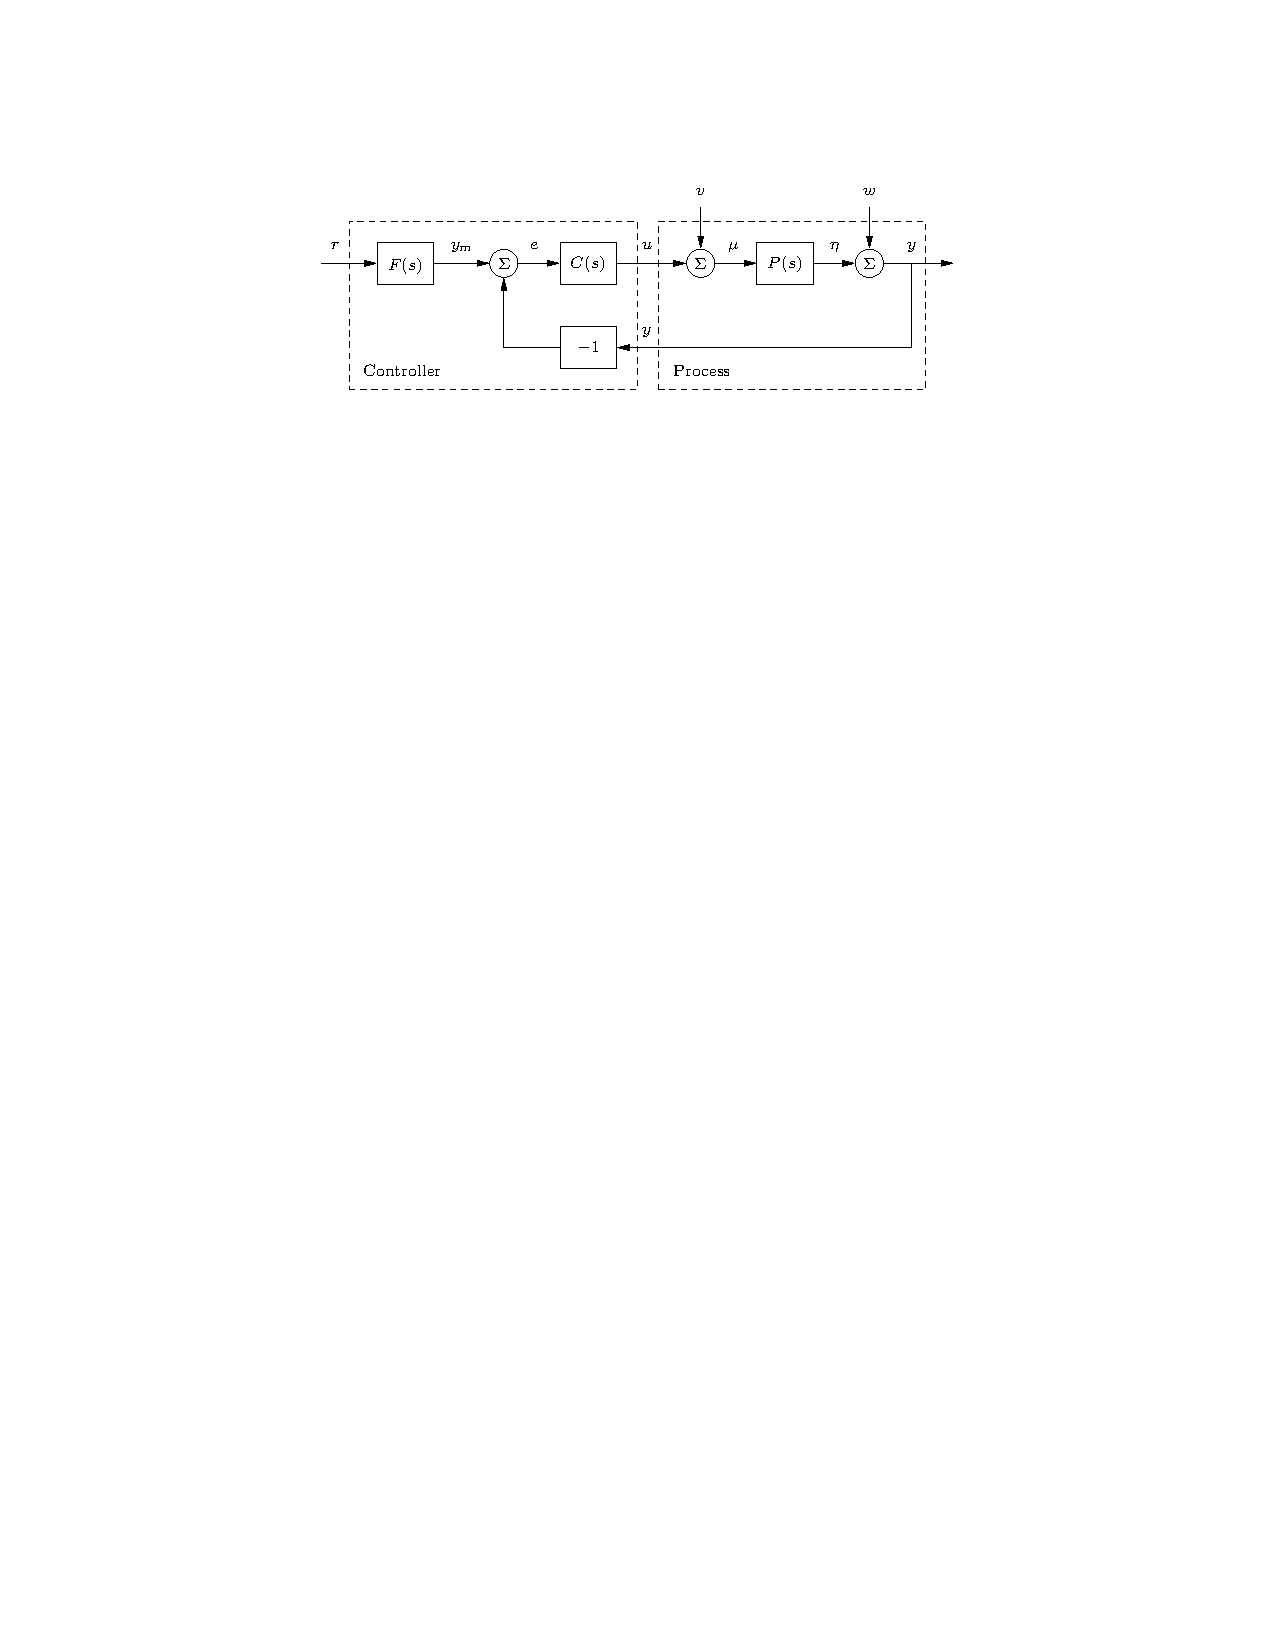
\includegraphics[width=10cm]{figure12.1}
	\textbf{Figure 12.1:} Block diagram of a control system with two degrees of freedom.
\end{figure}
\end{frame}

\begin{frame}{Goals of a control system}
\begin{itemize}
	\item Our goal is to make the process output $\eta$ track the reference signal $r$
	\item The process is a system with three inputs (control input $u$, load disturbance $v$, measurement noise $w$) and one output (measured signal $y$)
	\item The controller is a system with two inputs (measured signal $y$, reference signal $r$)  and one output (control signal $u$)
	\item We may investigate the relations between all signals by expressing them as transfer functions (of all external inputs $r$, $v$, $w$)
\end{itemize}
\end{frame}


\begin{frame}{Transfer functions}
\begin{itemize}
	\item The table below summarises all relevant transfer functions
	\item Many appear more than once and we can therefore direct our focus to a subset
\end{itemize}

	\centering
	\Large{
	\begin{table}
		\begin{tabular}{ccccc| c}
			\hline $y$ & $u$ & $e$ & $\mu$ & $\eta$ & \\
			\hline $\frac{P C F}{1+P C}$ & $\frac{C F}{1+P C}$ & $\frac{F}{1+P C}$ & $\frac{C F}{1+P C}$ & $\frac{P C F}{1+P C}$ & $r$\\
			$\frac{P}{1+P C}$ & $\frac{-P C}{1+P C}$ & $\frac{-P}{1+P C}$ & $\frac{1}{1+P C}$ & $\frac{P}{1+P C}$ & $v$\\
			$\frac{1}{1+P C}$ & $\frac{-C}{1+P C}$ & $\frac{-1}{1+P C}$ & $\frac{-C}{1+P C}$ & $\frac{-P C}{1+P C}$ & $w$ \\
			\hline
		\end{tabular}\\
		\vspace{.5cm}
		\normalsize{\textbf{Table 12.1:} Transfer functions relating the signals of the control system in Figure 12.1.}
\end{table}}
\end{frame}

\SUBCONCEPT{Gang of Six}

\begin{frame}{Select transfer functions}
\begin{itemize}
\item The Gang of Six transfer functions are
\[ G_{yr} = \frac{PCF}{1+PC}, \quad -G_{uv} = \frac{PC}{1+PC}, \quad G_{yv} = \frac{P}{1+PC},\]
\[G_{ur} = \frac{CF}{1+PC}, \quad -G_{uw} = \frac{C}{1+PC}, \quad G_{yw} = \frac{1}{1+PC}.\]

\item The response of the system to load disturbances and measurement noise is of importance for robustness in practice and these transfer functions are known as the sensitivity functions (or the Gang of Four)
\end{itemize}
\end{frame}

\begin{frame}{Sensitivity - Gang of Four}
\begin{itemize}
	\item The sensitivity function is 
	\[S=\frac{1}{1+PC}\]
	\item The load (or input) sensitivity function is 
	\[PS=\frac{P}{1+PC}\]
	\item The complementary sensitivity function is 
	\[T=\frac{PC}{1+PC}\]
	\item The noise (or output) sensitivity function is
	\[CS = \frac{C}{1+PC}\]
\end{itemize}
\end{frame}

\begin{frame}{Design of controllers}
\begin{itemize}
	\item The Gang of Four captures the response of the system to disturbances, which assists in the design of the controller $C$
	\item The remaining two transfer functions of the Gang of Six capture the relationship between the reference signal and hte measured output, which can be designed by $F$
	\item If all of the Gang of Four transfer functions are stable, the feedback system is said to be \textit{internally stable}
\end{itemize}
\end{frame}

\begin{frame}{Sensitivity and its complement}
\begin{itemize}
	\item The sensitivity function $S$ determines the attenuation of load disturbances
	\item The complementary sensitivity function $T$ determines robustness to measurement noise
	\item The sensitivity functions have the property that $S+T=1$ (this is why $T$ is called complementary sensitivity)
	\item Therefore, there are unavoidable trade-offs between performance and disturbance/noise attenuation (we can't make both $|S|$ and $|T|$ zero at the same time)
	\item Typically disturbances are low frequency and measurement noise is high frequency 
\end{itemize}
\end{frame}

\SUMMARYFRAME
\FINALE

\end{document}
